\chapter{Selective cross-linking of coinciding protein assemblies by in-gel cross-linking mass-spectrometry} \label{ch-2}

{
Johannes F. Hevler\textsuperscript{1,2*}, Marie V. Lukassen\textsuperscript{1,2*}, Alfredo Cabrera-Orefic\textsuperscript{3}, Susanne Arnold\textsuperscript{3}, Matti F. Pronker\textsuperscript{1,2}, Vojtech Franc\textsuperscript{1,2} and Albert J.R. Heck\textsuperscript{1,2,\Letter} 

\vspace{0.3cm}
\textbf{\emph{The EMBO Journal}} (2021), 40:e106174, doi:10.15252/embj.2020106174\\

\footnotesize
\vspace{0.3cm}
\begin{tabular}[t]{p{0.01\textwidth}p{0.90\textwidth}}
1 &  Biomolecular Mass Spectrometry and Proteomics, Bijvoet Center for Biomolecular Research and Utrecht Institute for Pharmaceutical Sciences, University of Utrecht,
Padualaan 8, 3584 CH Utrecht, The Netherlands\\
2 & Netherlands Proteomics Center, Padualaan 8, 3584 CH Utrecht, The Netherlands\\
3 & Radboud Institute for Molecular Life Sciences, Radboud University Medical Center, 6525 GA Nijmegen, The Netherlands.\\
\textsuperscript{*} & These authors contributed equally to this work\\
\end{tabular}
\\
}

\newpage
\begin{abstract101} 
Cross-linking mass spectrometry has developed into an important method to study protein structures and interactions. The in-solution cross-linking workflows involve time and sample consuming steps and do not provide sensible solutions for differentiating cross-links obtained from co-occurring protein oligomers, complexes, or conformers. Here we developed a cross-linking workflow combining blue native PAGE with in-gel cross-linking mass spectrometry (IGX-MS). This workflow circumvents steps, such as buffer exchange and cross-linker concentration optimization. Additionally, IGX-MS enables the parallel analysis of co-occurring protein complexes using only small amounts of sample. Another benefit of IGX-MS, demonstrated by experiments on GroEL and purified bovine heart mitochondria, is the substantial reduction of undesired over-length cross-links compared to in-solution cross-linking. We next used IGX-MS to investigate the complement components C5, C6, and their hetero-dimeric C5b6 complex. The obtained cross-links were used to generate a refined structural model of the complement component C6, resembling C6 in its inactivated state. This finding shows that IGX-MS can provide new insights into the initial stages of the terminal complement pathway.
\end{abstract101}

\newpage

\section{Introduction}
Over the last decades, bimolecular mass spectrometry (MS), with its ability to analyze low amounts of samples with high speed and sensitivity, has evolved into a central pillar beneficial for integrative structural biology \cite{de_Souza_2020, Kaur_2019, Lossl_2016, Robinson_2019}. The structural MS toolbox contains multiple complementary approaches. Next to native MS and top-down MS, a variety of peptide-centric MS methods, such as thermal proteome profiling (TPP), limited proteolysis (LiP), hydrogen/deuterium exchange (HDX) MS and chemical cross-linking MS (XL-MS or CLMS), have emerged and enabled structural studies of a wide range of biomolecules \cite{Feng_2014, Heck_2008, Leitner_2010, Savitski_2014, Zheng_2019}. With recent advances in instrumentation, sample preparation, and data analysis, especially XL-MS has started to fulfill its potential to complement well established structural methods such as X-ray crystallography, nuclear magnetic resonance spectroscopy (NMR), and cryo-electron microscopy (cryo-EM) \cite{Leitner_2016, Matthew_Allen_Bullock_2016, Rappsilber_2011}. XL-MS has a particular utility to capture protein-protein interactions in solution by measuring spatial distance restraints, mirroring structural conformations of intact proteins. Concomitantly, a wide range of chemical cross-linkers have been explored so far, often relying on similar chemical principles \cite{Sinz_2003, Steigenberger_2020}. Most used cross-linkers are small, homo-bifunctional reagents, with two reactive moieties capable of covalently binding two nearby amino acids. The reactive groups are separated by a spacer arm of varying lengths, which can be gas-phase cleavable or non-cleavable, thereby determining different MS data acquisition methods \cite{Kao_2011, Leitner_2010, Muller_2010, Staros_1982}. Recent advances in search engines for more efficient identification of cross-linked peptides allowed structural studies of purified proteins or protein complexes, as well as large scale experiments with more complex samples like purified organelles or cell lysates, using buffer systems which aim to meet physiological relevant conditions \cite{Beveridge_2020, Chen_2019a, Gotze_2019, Klykov_2018}. A typical XL-MS workflow begins with the optimization of the cross-linker concentration. Next, a protein mixture is incubated with the cross-linking reagent, and the reaction is subsequently quenched to prevent the generation of unwanted random protein contacts. After (tryptic) digestion, cross-linked peptides are subjected to various pre-fractionation steps or enrichment strategies to distinguish them from the vast majority of unmodified peptides. Cross-linked residues are eventually identified using dedicated XL-MS search algorithms, providing structural information in the form of distance restraints, which can be utilized to guide computational homology modeling, refinement of flexible regions within structural models, protein-protein docking and the generation of protein interaction networks \cite{Albanese_2020, Bullock_2018, Iacobucci_2019, Kim_2018, Ryl_2020}. Currently, technological developments in XL-MS aim to further improve the cross-linking reaction efficiency and detection. The research is mainly focused on sample preparation techniques, MS fragmentation and enrichment strategies, data acquisition and analysis of cross-linked peptides, as well as the design of novel cross-linkers \cite{Chen_2019b, Dau_2019, Iacobucci_2018, Leitner_2012, Liu_2017, Mendes_2019, Steigenberger_2019}.\\
Although the latest advances significantly revised and reformed the field of XL-MS, some challenges remain. A central problem of XL-MS data analysis is the occurrence of both false-positive and false-negative cross-link identifications. Especially, the existence of proteins with highly dynamic/flexible conformations and the presence of co-occurring alike protein complexes (e.g., protein oligomers and co-occurring complexes sharing distinct sub-units) significantly complicate the analysis by current in-solution XL-MS approaches. Interaction specific cross-links are relevant as structural changes can be triggered by the presence of a binding partner or the environment, thereby eventually displaying a physiological relevant protein conformation \cite{de_Souza_2020, Feng_2014, Mannige_2014, Uversky_2011}. Additionally, when using too high cross-linker concentrations or too high protein concentrations, undesired artificial interactions are likely being picked up by XL-MS. In-solution XL-MS experiments, therefore, need careful experimental optimization of, in particular, the concentration of the proteins and the cross-linker. Unfortunately, these steps require considerable sample amounts (tens of micrograms) and extra experimental time.\\
Here we describe an alternative approach, performing in-gel cross-linking mass spectrometry (IGX-MS), re-discovering the great separation power of gel-electrophoresis. Prior to cross-linking, we load the samples and perform blue native polyacrylamide gel

\begin{figure*}[hbt!]
\center
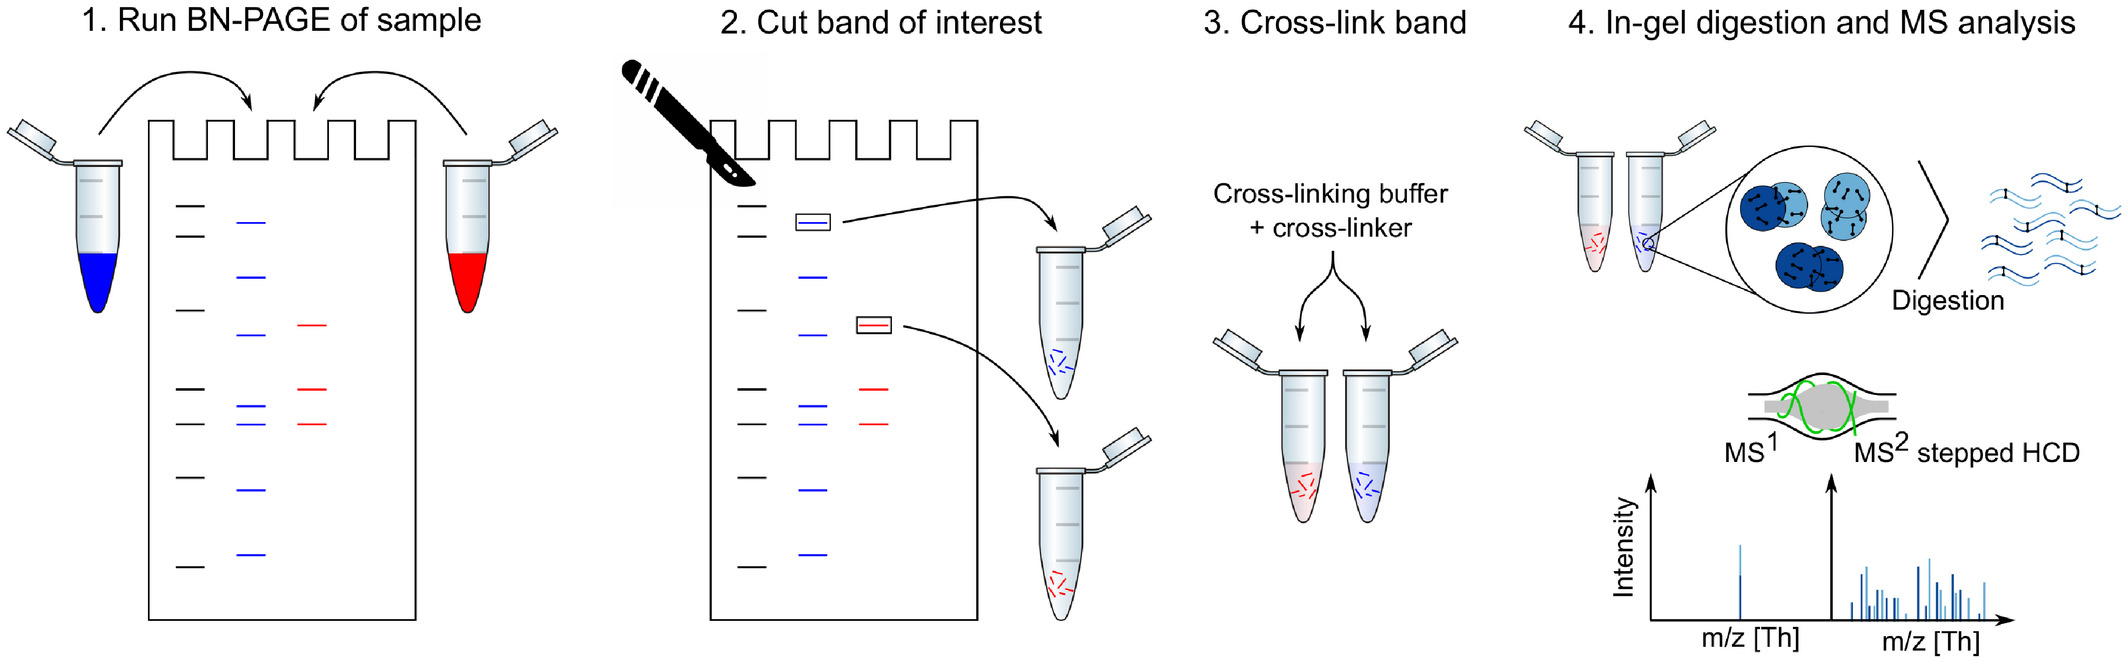
\includegraphics[width=\textwidth]{Chapter.2/Figures/Fig1.jpg} 
\caption{\textbf{Combining BN-PAGE with IGX-MS.} In the first step, proteins and their assemblies are loaded and separated by BN-PAGE. The bands representing different protein assemblies are visualized after running the gel with Coomassie in the upper running buffer. The band(s) of interest are then excised from the gel and incubated with a cross-linking reagent in the cross-linking buffer. The cross-linking reaction is quenched and subsequently subjected to standard in-gel digestion. The extracted peptides are finally analyzed using cross-linking optimized parameters for the MS analysis.}
\label{fig:ch2_fig1}
\end{figure*}

electrophoresis (BN-PAGE), allowing the separation of distinct structural states of the proteins or protein complexes. The distinct bands are subsequently excised and cross-linked in the gel, enabling the measurement of conformation- and interaction-specific cross-links and derived distance restraints (\textbf{\autoref{fig:ch2_fig1}}). We show that this IGX-MS workflow has certain advantages compared to the in-solution based XL-MS methods. These include, amongst other things, no need for cross-linker concentration optimization, generation of conformation-specific cross-links, and relatively low sample amount requirements. Moreover, through IGX-MS data obtained for several protein assemblies, we provide evidence that proteins retain not only their quarternary but also their secondary and tertiary native structural states under BN-PAGE separation. To directly compare IGX-MS with in-solution XL-MS, we selected, as a proof-of-concept, the 14-mer \emph{Escherichia coli} GroEL chaperone and different respiratory chain complexes (super complex 1, complex I and complex V) from solubilized bovine heart mitochondria (BHM). Our experiments demonstrated that IGX-MS can accurately target specific subcomplexes co-existing in the protein complex mixtures and substantially reduce the number of (potentially false) over-length cross-links. Ultimately, we applied the optimized IGX-MS to investigate structures of the terminal complement proteins C5 and C6, which are involved in the initial steps towards the assembly of membrane attack complex (MAC). Our cross-linking data lead us to propose a refined alternative structural conformation of the complement component C6, providing new insights into the terminal complement pathway. In summary, our data show that BN-PAGE-based IGX-MS is a powerful tool, allowing the efficient generation of compositional- and interaction-specific distance constraints, with the potential of refining structural models of a large variety of protein assemblies, even when they co-occur in solution.

\section{Results}
\subsection{BN-PAGE forms the basis for IGX-MS}
Blue native polyacrylamide gel electrophoresis, BN-PAGE, has proven to be a robust and sensitive method for separating protein complexes from various sample types. It requires only minimal sample amounts to sensitively estimate native protein molecular weights (Mw), respective compositional states, and protein-protein interactions. Further, proteins and protein complexes are thought to maintain not only their overall quarternary structural organization in the gel but also their secondary and tertiary structural organization, as they can still, after that, be subjected to further structural and functional analysis (2D crystallization, cryo-EM, in-gel activity assay) \cite{Poetsch_2000, Schafer_2006, Wittig_2007}.\\
Here, we combine BN-PAGE with XL-MS to efficiently isolate and investigate co-occurring protein oligomeric states and sub-complexes. We first determined whether proteins and protein complexes can be cross-linked in a BN gel. For this, 10 µg of purified E. Coli GroEL diluted in a Tris buffer was subjected to BN-PAGE as described previously \cite{Wittig_2006}. Bands corresponding to the native 14-mer GroEL (MW = 800 kDa) were excised from the BN-PAGE (\textbf{\autoref{fig:ch2_app_fig1}A}), and further, cut into small pieces and incubated with or without the cross-linker reagent DSS. Next, GroEL was extracted from the gel pieces and subsequently loaded onto a reducing SDS-PAGE (\textbf{\autoref{fig:ch2_app_fig1}B}). The control lane (no cross-linker) revealed only one distinct band at 57 kDa representing the GroEL monomers. In contrast, the BN-PAGE band that was incubated with DSS showed several additional high-molecular-weight bands above 100 kDa, indicating the successful cross-linking of GroEL subunits. Notably, the initial sample buffer (Tris) is incompatible with amine-reactive cross-linkers, as it contains primary amines that compete with the primary amines of Lysine residues, thereby significantly reducing the cross-link efficiency. Successful cross-linking of GroEL in-gel highlights the buffer exchange capacity of the BN-PAGE system, making additional buffer exchange steps (e.g., using molecular weight cut-off filters or dialysis), which would be required for in-solution cross-linking and eventually result in loss of sample, obsolete.

\subsection{IGX-MS optimization is straightforward}
To prevent protein precipitation caused by over cross-linking, standard in-solution XL-MS crucially depends on using the optimal cross-linker concentration. For this, a subset of sample needs to be incubated with varying cross-linker concentrations prior to the experiment and subsequently analyzed by gel electrophoresis. The time and sample consuming optimization step led us to investigate the effect of varying cross-linker concentrations for IGX-MS experiments. GroEL was subjected to BN-PAGE, and relevant bands were cross-linked using the two different cross-linking reagent DSS and DSSO varying in five concentration steps from 0.5 to 5 mM. After quenching the cross-linking reaction with Tris, the protein-containing bands were prepared for MS analysis following a standard in-gel digestion procedure. Cross-links obtained for DSS and DSSO, and each concentration were validated by mapping them onto the GroEL structure (PDB ID: 1KP8), and lysine C\(\alpha\)-C\(\alpha\) distances were obtained (textbf{Dataset EV1}). The distance distribution for both cross-linkers was highly similar at all used concentrations, and almost no cross-link distances over 30 Å were observed across the varying concentrations, indicating that IGX-MS is highly resistant against over cross-linking of proteins (\textbf{\autoref{fig:ch2_fig2}A}). Our data suggest that IGX-MS is also less hampered by\\

\begin{figure*}[hbt!]
\center
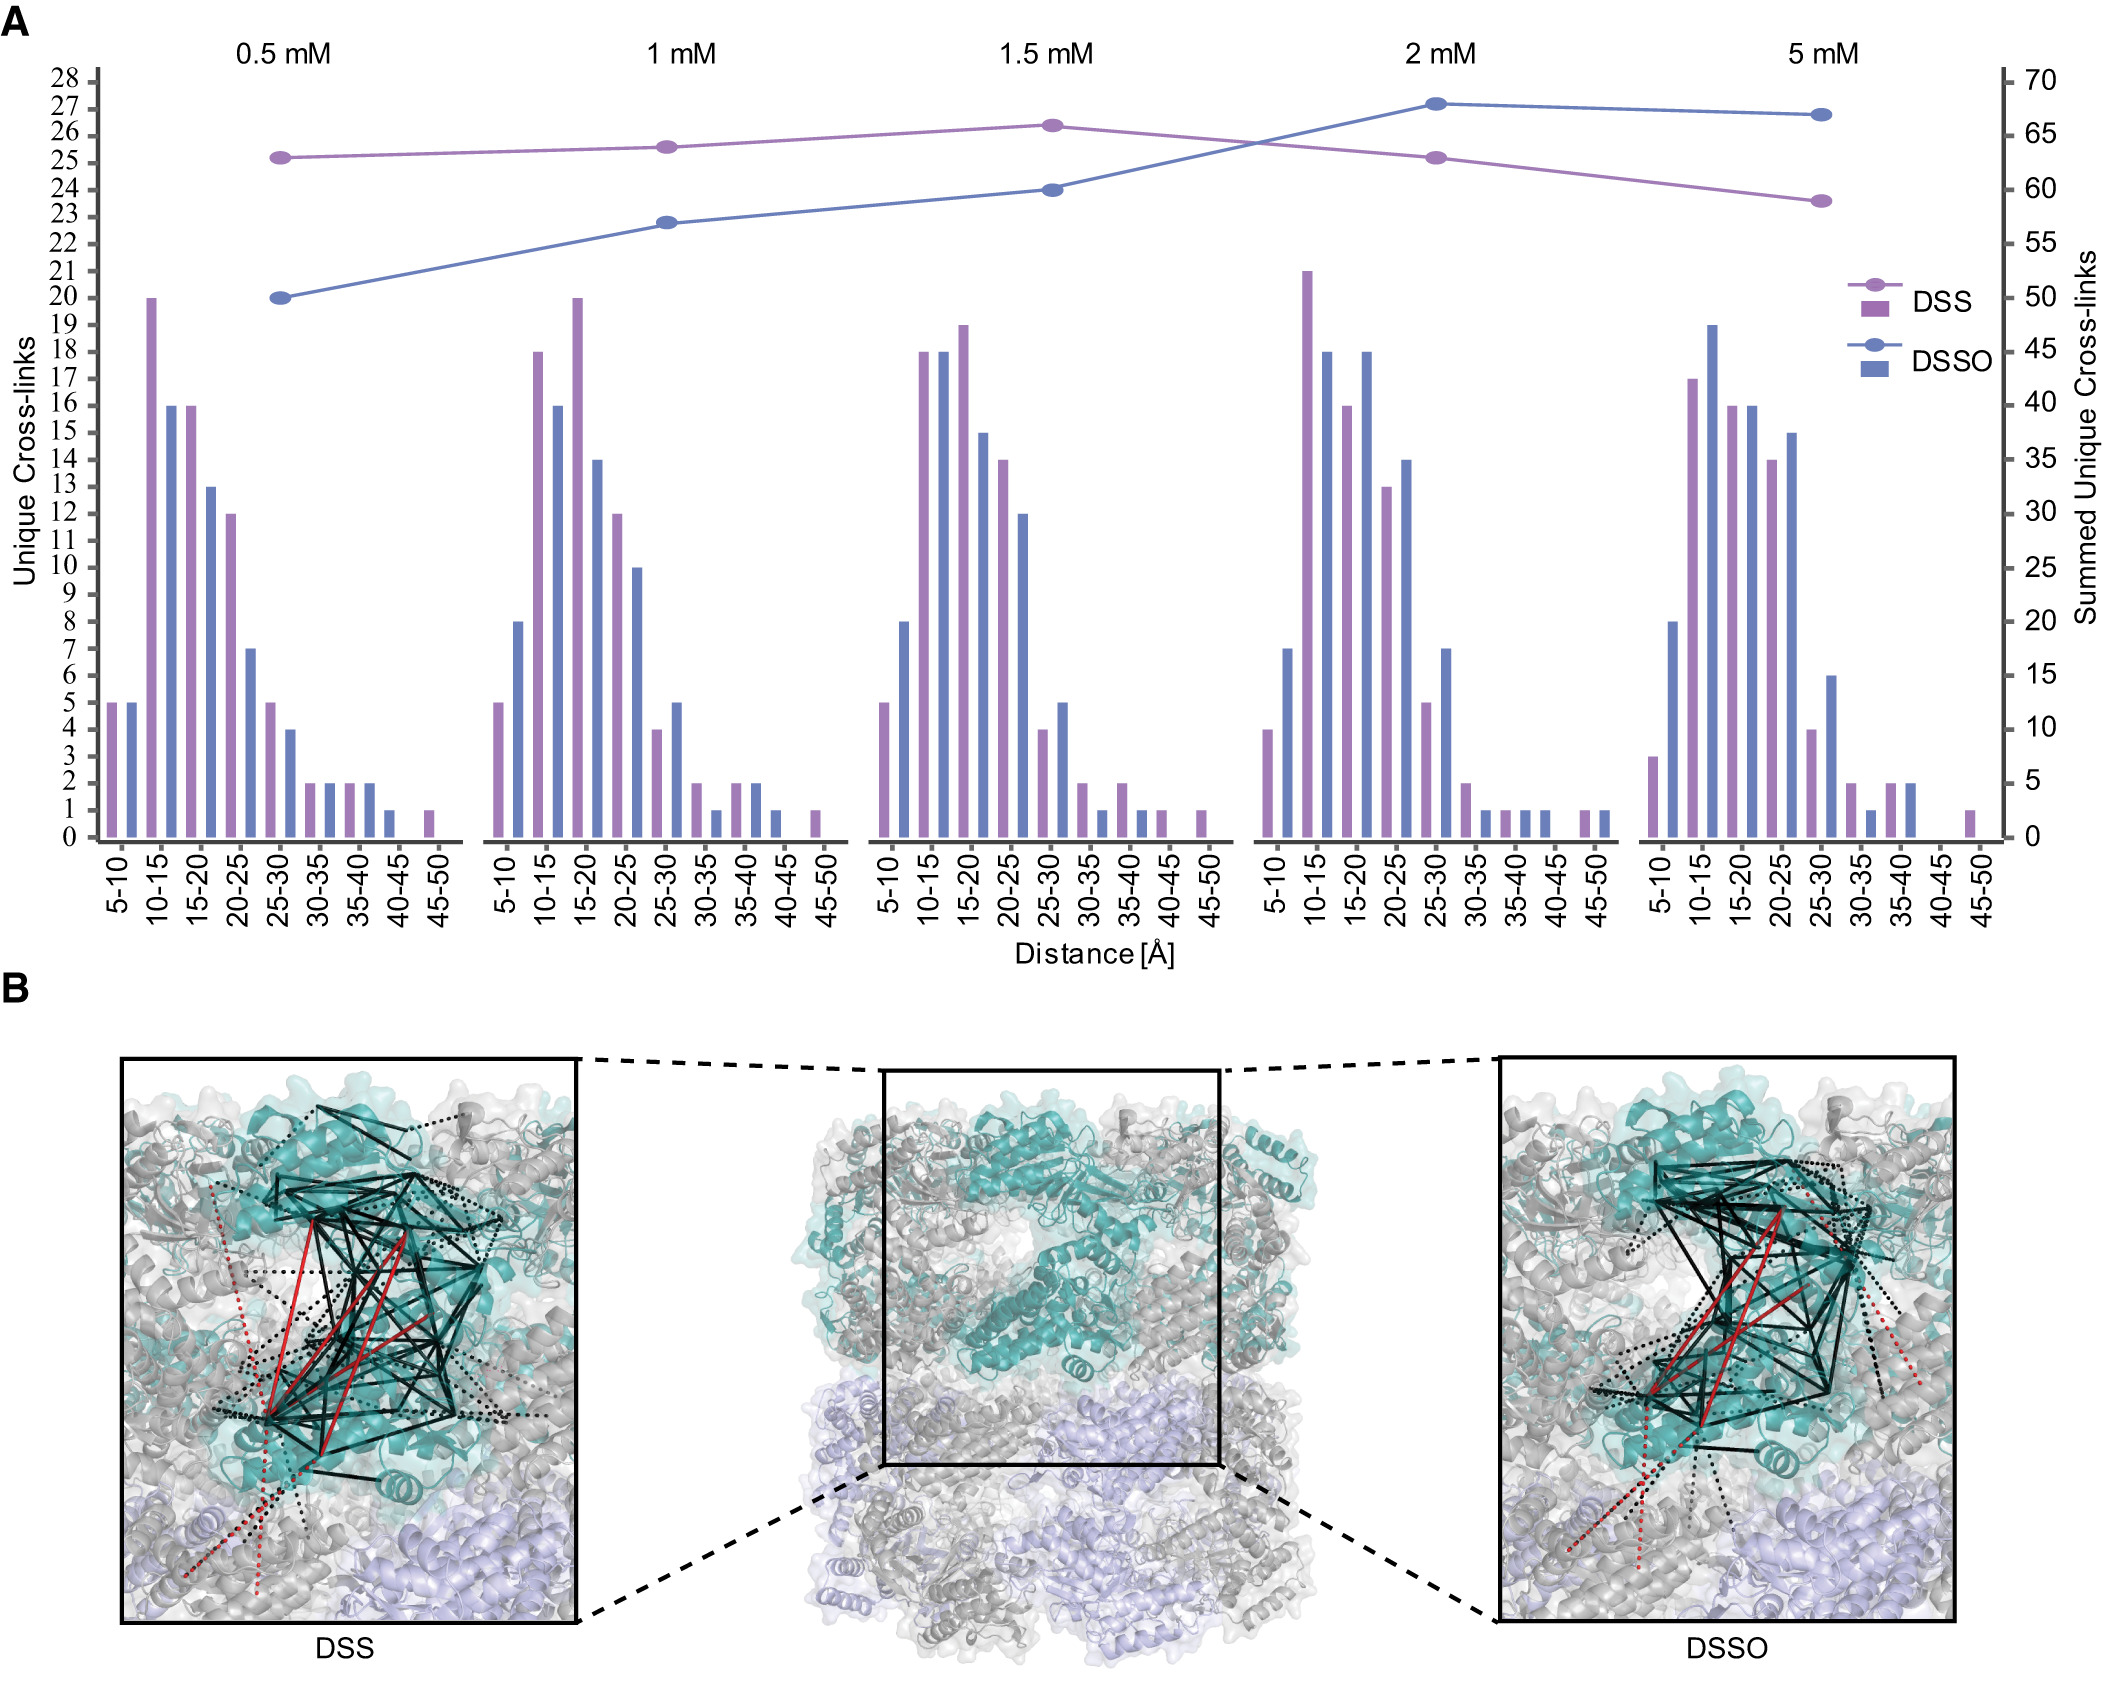
\includegraphics[width=\textwidth]{Chapter.2/Figures/Fig2.jpg} 
\caption{\textbf{IGX-MS of GroEL using either DSS or DSSO at varying concentrations.} \textbf{A.} \emph{Escherichia coli} GroEL was cross-linked by IGX-MS using either DSS or DSSO at concentrations ranging from 0.5 to 5 mM. The identified cross-links were placed on the reported GroEL structure (PDB ID:1KP8), whereby the number of unique cross-linked lysine C\(\alpha\)-C\(\alpha\) distances (using the left y-axis) were binned and as shown in bars. The summed number of unique cross-links obtained at each concentration is shown in lines using the right y-axis. \textbf{B.} Cross-links obtained by IGX-MS using DSS or DSSO plotted onto one subunit of GroEL (intra-links; solid lines) (PDB ID:1KP8) and neighboring subunits (inter-links; dashed lines). Cross-links agreeing with the set distance restraint of 30 Å are colored black, links exceeding the restraint are colored red. Data information: The presented data is summed from triplicates.}
\label{fig:ch2_fig2}
\end{figure*}

unspecific cross-links. We also observed that the total number of unique cross-links was not affected by the concentration of DSS, and only marginally effected for DSSO as the obtained cross-links are slightly lower for concentrations below 2 mM (\textbf{\autoref{fig:ch2_fig2}A}). However, no significant difference was detected between 2 mM and 5 mM (\textbf{\autoref{fig:ch2_fig2}A}). The cross-linked sites onto the GroEL structure showed good consistency in cross-linked regions for both DSS and DSSO experiments (\textbf{\autoref{fig:ch2_fig2}B}, textbf{Dataset EV1}). Finally, we compared the cross-linking results for each cross-linker and concentration across the three replicates, demonstrating excellent reproducibility of the IGX-MS experiments (\textbf{\autoref{fig:ch2_app_fig2}}). Based on these results, a DSS concentration of 1.5 mM and a DSSO concentration of 2 mM (\textbf{\autoref{fig:ch2_fig2}A}) were used for the subsequent experiments.

\subsection{Direct comparison of IGX-MS and in-solution XL-MS}
BN-PAGE facilitates the distinction of oligomeric states, but it can also be particularly useful when protein complexes are reconstituted. In such experiments, one or more of the subunits may be (unwillingly) in excess. These preparations can then lead to false cross-link interpretations, as especially intra cross-links can originate from the free monomer subunit or subunit in the complex (which may exhibit another conformation). By comparing IGX-MS and in-solution XL-MS of GroEL, we aimed to access the relevance of this additional separation aspect and confirm that proteins maintain their native structural integrity during in-gel separation. First, for in-solution cross-linking, GroEL diluted in Tris buffer was buffer exchanged to PBS, and subsequently, the optimal cross-linker concentration was determined by SDS-PAGE to avoid over cross-linking (\textbf{\autoref{fig:ch2_app_fig3}A}). Next, the in-solution XL-MS sample was cross-linked with DSS, while the IGX-MS sample was cross-linked with both DSS and DSSO. Subsequent comparison of DSS- and DSSO-in-gel cross-linked samples showed a 53 \% overlap of identified cross-linked sites. Next, we directly compared in-solution XL-MS and IGX-MS. Although a significant number (60 \%) of DSS-in-gel cross-links was also detected by in-solution XL-MS (\textbf{\autoref{fig:ch2_fig3}A}), in-solution XL-MS resulted in a seemingly higher total number of unique cross-links compared to IGX-MS. First, we ruled out that the higher number of unique cross-links in-solution could be explained by insufficient extraction of long peptides from the gel, based on the observation that the detected cross-linked peptides displayed a similar length distribution (\textbf{\autoref{fig:ch2_app_fig3}B}). Plotting all the cross-links onto the GroEL structure revealed that a large portion of the "exclusive" in-solution cross-links originated from paired lysine residues separated by more than 30 Å, our distance cut-off. In contrast, virtually all IGX-MS cross-links remained below this cut-off (\textbf{\autoref{fig:ch2_fig3}B}, \textbf{Dataset EV1}). Therefore, we are convinced that the BN-PAGE gel separation removes the co-analysis of co-occurring protein assembly states and higher-order protein aggregates. The latter often leads to the observation of over-length cross-links in solution. Further, mapping and directly comparing the overlapped cross-links between the IGX-MS and in-solution XL-MS revealed high consistency of cross-linked sites, supporting that GroEL preserved its native conformation in the gel.

\begin{figure*}[hbt!]
\center
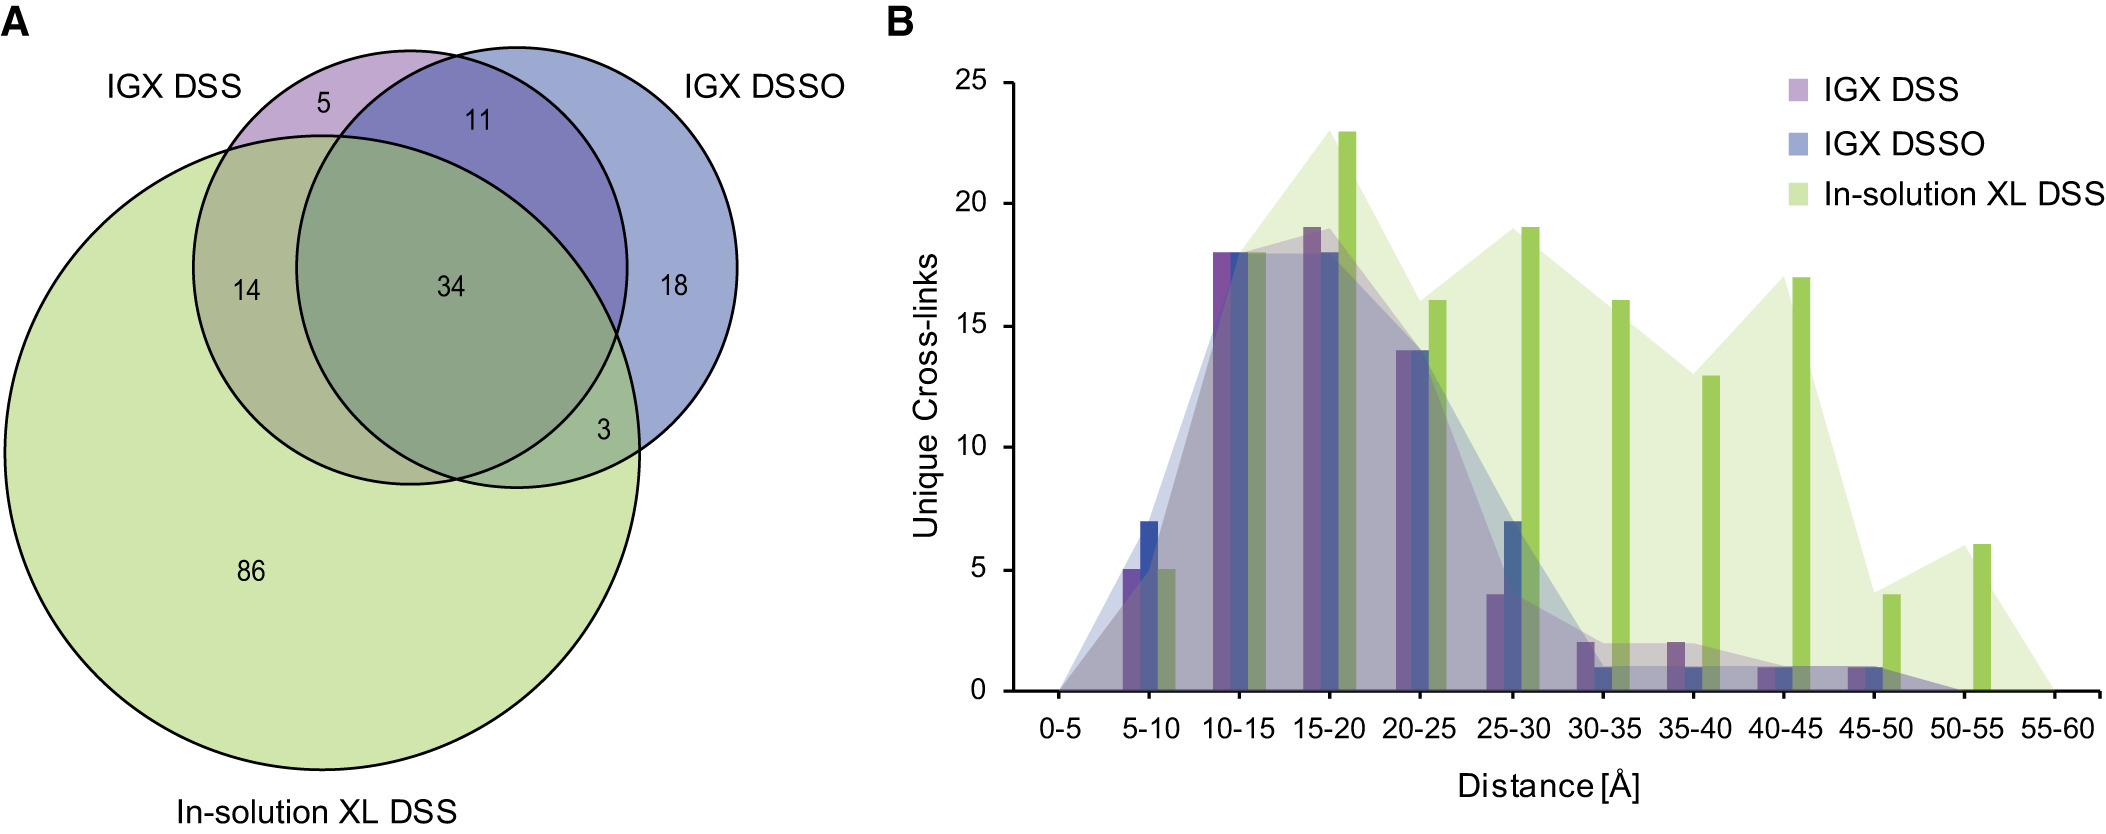
\includegraphics[width=\textwidth]{Chapter.2/Figures/Fig3.jpg} 
\caption{\textbf{Comparison of IGX-MS and in-solution XL-MS of GroEL.} \textbf{A.} \emph{Escherichia coli} GroEL was subjected to in-solution XL-MS using 0.75 mM DSS. The resulting cross-links were compared to cross-links obtained by IGX-MS using DSS (1.5 mM) or DSSO (2 mM). The Venn diagram shows the overlap in the cross-links identified. \textbf{B.} Distribution of lysine C\(\alpha\)-C\(\alpha\) distances of unique cross-links identified by IGX-MS (DSS or DSSO) or in-solution XL-MS plotted on the GroEL structure (PDB ID:1KP8). Data information: The presented data is summed from triplicates.}
\label{fig:ch2_fig3}
\end{figure*}

\subsection{IGX-MS facilitates the analysis of distinct co-occurring assemblies}
Proteins in cells or extracted from various biological sources can be part of multiple different complexes. Whether a protein is a free monomer or part of one or more protein complexes can substantially affect its structure. The identification of distinctive structural states of a protein by XL-MS in solution is often hampered, especially when the "free" monomer co-exist with the same protein being part of one or more complexes. For this reason, we investigated whether IGX-MS can exclusively obtain cross-links for proteins in a single configuration of the complex. As a first test-sample, we incubated GroEL with one of its known natural unfolded substrates, namely the bacteriophage T4 capsid protein (gp23, 56 kDa). Following incubation of GroEL with unfolded gp23, we analyzed this sample by BN-PAGE and observed three distinctive bands, corresponding to free GroEL and GroEL with one or two copies of gp23 bound (\textbf{\autoref{fig:ch2_app_fig4}A}). That GroEL can bind two substrate molecules (in the cis and trans ring) agrees with previously reported data (van Duijn et al., 2006) and could be additionally confirmed by relative quantification of the subunits in the respective bands (\textbf{\autoref{fig:ch2_app_fig4}B}). In parallel cross-linking of each band, i.e., GroEL, GroEL:gp23 and GroEL:(gp23)2, with DSS, revealed interlinks between GroEL and gp23 exclusively in the middle and upper band whereby the primary inter-linked residues in GroEL were identified as K42, K122, and K272 (Dataset EV2). The site with most cross-links to gp23 was K272, located at the outer edge of the cavity (\textbf{\autoref{fig:ch2_app_fig4}C-D}). IGX-MS of each BN-PAGE bands enabled the identification of protein compositional specific distance restraints, which would have been impossible by in-solution XL-MS without additional experimental steps.
Next, we assessed the capabilities of IGX on a more complex sample and subjected 20 µg of purified bovine heart mitochondria (BHM), solubilized with digitonin, to BN-PAGE (Fig 4A). It is well-known that BN-PAGE can separate and visualize the different complexes of the mitochondrial respiratory chain, including many of the co-occurring super-complexes (Schagger and Pfeiffer, 2000). The band corresponding to the monomeric form of complex V (the well-studied ATP synthase, which can also be abundantly present in a V2 dimeric form), was excised and subjected to IGX-MS using DSS (Fig 4A). The detected cross-links were plotted onto the 3D structure (PDB ID: 5ARA) and compared to cross-links detected in a previously published data set from our lab, by in-solution XL-MS (Liu et al., 2018) (Fig 4B, Dataset EV3). Visualizing the detected IGX-MS- and in-solution XL-MS cross-linked regions revealed their high consistency, indicating that these membrane protein complexes largely retain their quarternary, tertiary, and secondary structures in the BN-PAGE gel. Similar to the previous in-solution XL-MS experiments, only solvent-accessible regions of complex V subunits (which in intact mitochondria are facing the matrix) were detected in the IGX data. Further, we found that ATP5IF, a known inhibitor of the ATPase, was associated with the monomeric ATP synthase (Fig 4C). Detected cross-links from the inhibitor to ATP5F1E, ATP5F1D, ATP5F1C, and ATP5F1B agree with the previously reported binding interface of ATP5IF and the ATPase (Gledhill et al., 2007). In-solution XL-MS resulted in a higher number of unique cross-links (248 vs. 53 for IGX). However, like for GroEL, the C\(\alpha\)-C\(\alpha\) distance distribution revealed that many in-solution XL-MS cross-links are well above the 30 Å cut-off (149 unique cross-links). The IGX-MS cross-links are predominantly below this set cut-off (only two unique cross-links above), highlighting the accordance of the IGX-MS generated restrains with the previously published structure of monomeric ATPase (Fig 4D, Dataset EV 3). We argue that some of these over-length cross-links detected by in-solution XL-MS may originate from co-occurring dimeric complex V or other ATPase conformations induced upon binding of one (or several) of its many previously identified interactors (Liu et al., 2018; Ryl et al., 2020; Schweppe et al., 2017). Additionally, IGX-MS generated cross-links exclusively describe the interaction of ATP5IF to monomeric ATP synthase. In contrast, in-solution XL-MS generated cross-links most-likely reflect distance restraints for different assembly states of ATP synthase (e.g., monomeric/dimeric ATP synthase with and without ATP5IF). To further showcase the ability of IGX-MS to generate assembly state-specific cross-links, bands corresponding to monomeric complex I (CI) and the super complex 1 (S1) were excised and subjected to IGX-MS using DSS (Figure EV1A). For both assembly states, a similar interaction network between the CI subunits was observed (Figure EV1A, Dataset EV3), revealing subunits that are in close proximity to each other in assembled CI (PDB ID: 5GUP). Cross-links detected for the super complex 1 (S1) revealed inter-complex links between NDUFB4 (a subunit of complex I), UQCRC1, UQCRB (both subunits of complex III), COX7A1, and COX5B (both subunits of complex IV). This data agrees with the previously published structure (Wu et al., 2016), which identified respective subunits in the interface regions of S1 (Figure EV1A, PDB ID: 5GUP). As reported for the ATP synthase, IGX-MS data for CI (monomeric and S1) closely resembles the previously reported in-solution XL-MS data (Liu et al., 2018) (Dataset EV3). Moreover, the targeted approach of IGX-MS allowed us to distinguish cross-links coming from monomeric CI or CI as part of S1, whereas in-solution XL-MS data represents a mixture of all the different assembly states (e.g., monomeric and S0-S4) (Fig 4A, Figure EV1B).
In summary, comparing the IGX-MS and in-solution XL-MS cross-links for mitochondrial complex V, complex I and S1 highlights the capability of IGX-MS to generate sufficient, reliable and assembly-specific distance restraints.


\clearpage
\begin{subappendices}
    \counterwithin{figure}{section}
    \section{Supplementary Material}

    \begin{figure*}[hbt!]
        \center
        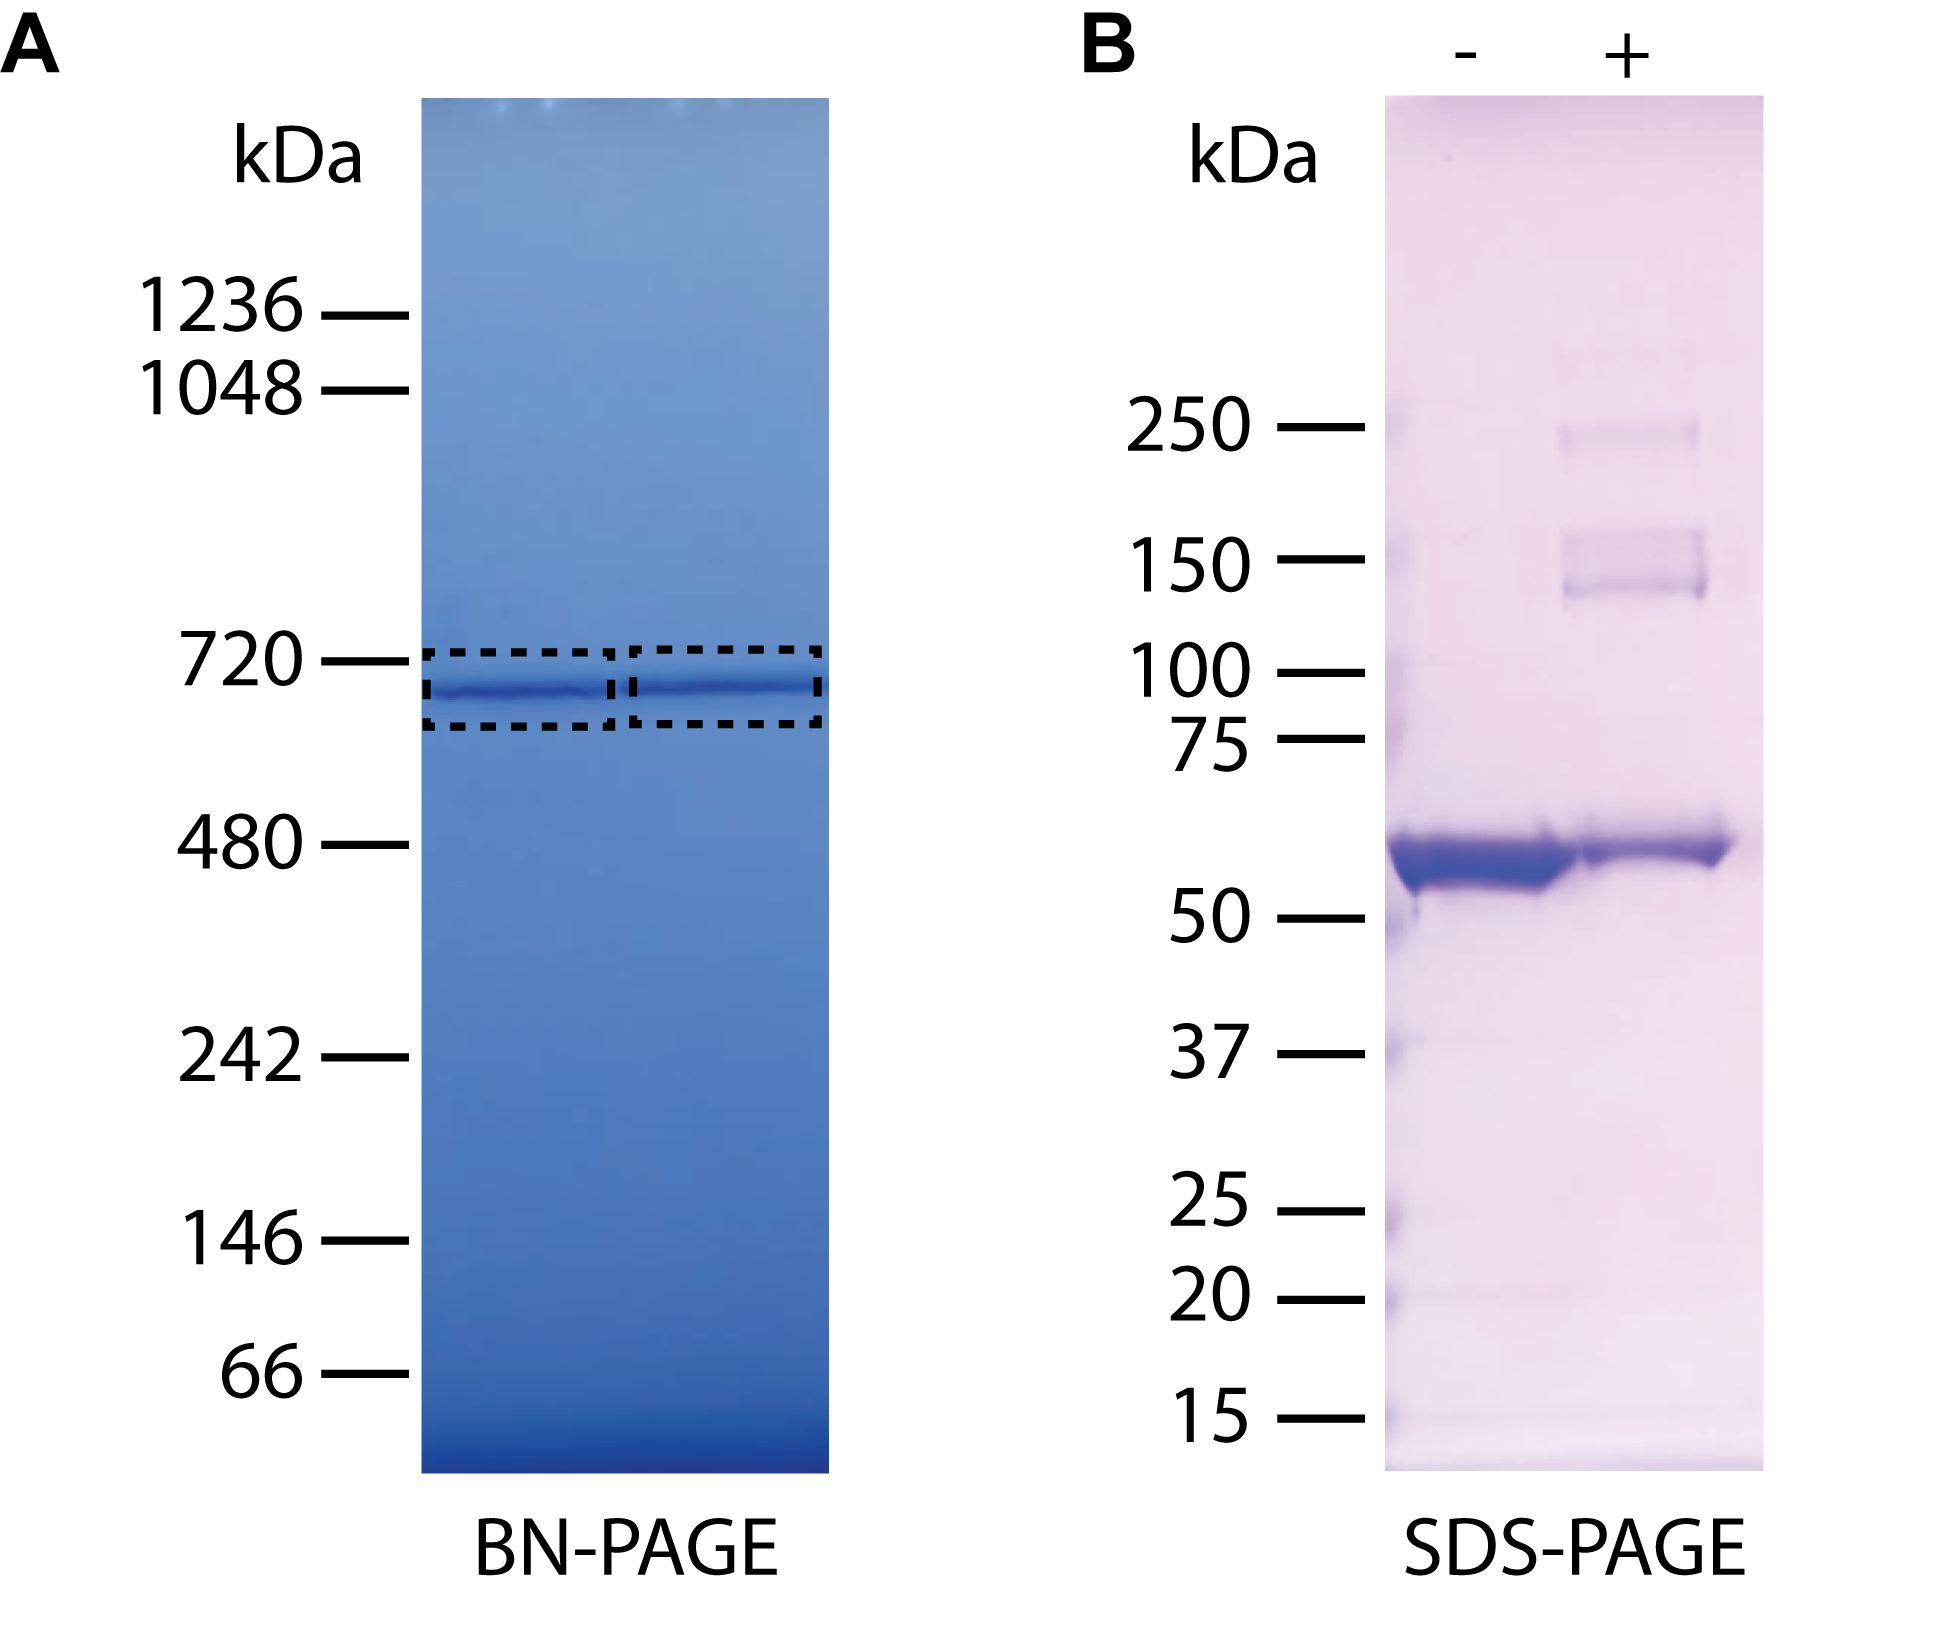
\includegraphics[width=0.5\textwidth]{Chapter.2/Figures/SI_Fig1.png} 
        \caption{\textbf{Combining BN-PAGE with IGX-MS.} \textbf{A.} A.	BN-PAGE of E. Coli (10 µg). Respective bands (dashed boxes) were excised and incubated with or without the cross-linker DSS (1.5 mM). \textbf{B.} B.	SDS-PAGE of GroEL, extracted from respective gel band (see A). The non-cross-linked control (-) showed only a band at 57 kDa of the GroEL subunit, whereas the DSS-cross-linked sample (+) reveals several bands at higher Mw.}
        \label{fig:ch2_app_fig1}
    \end{figure*}

    \vspace{1cm}

    \begin{figure*}[hbt!]
        \center
        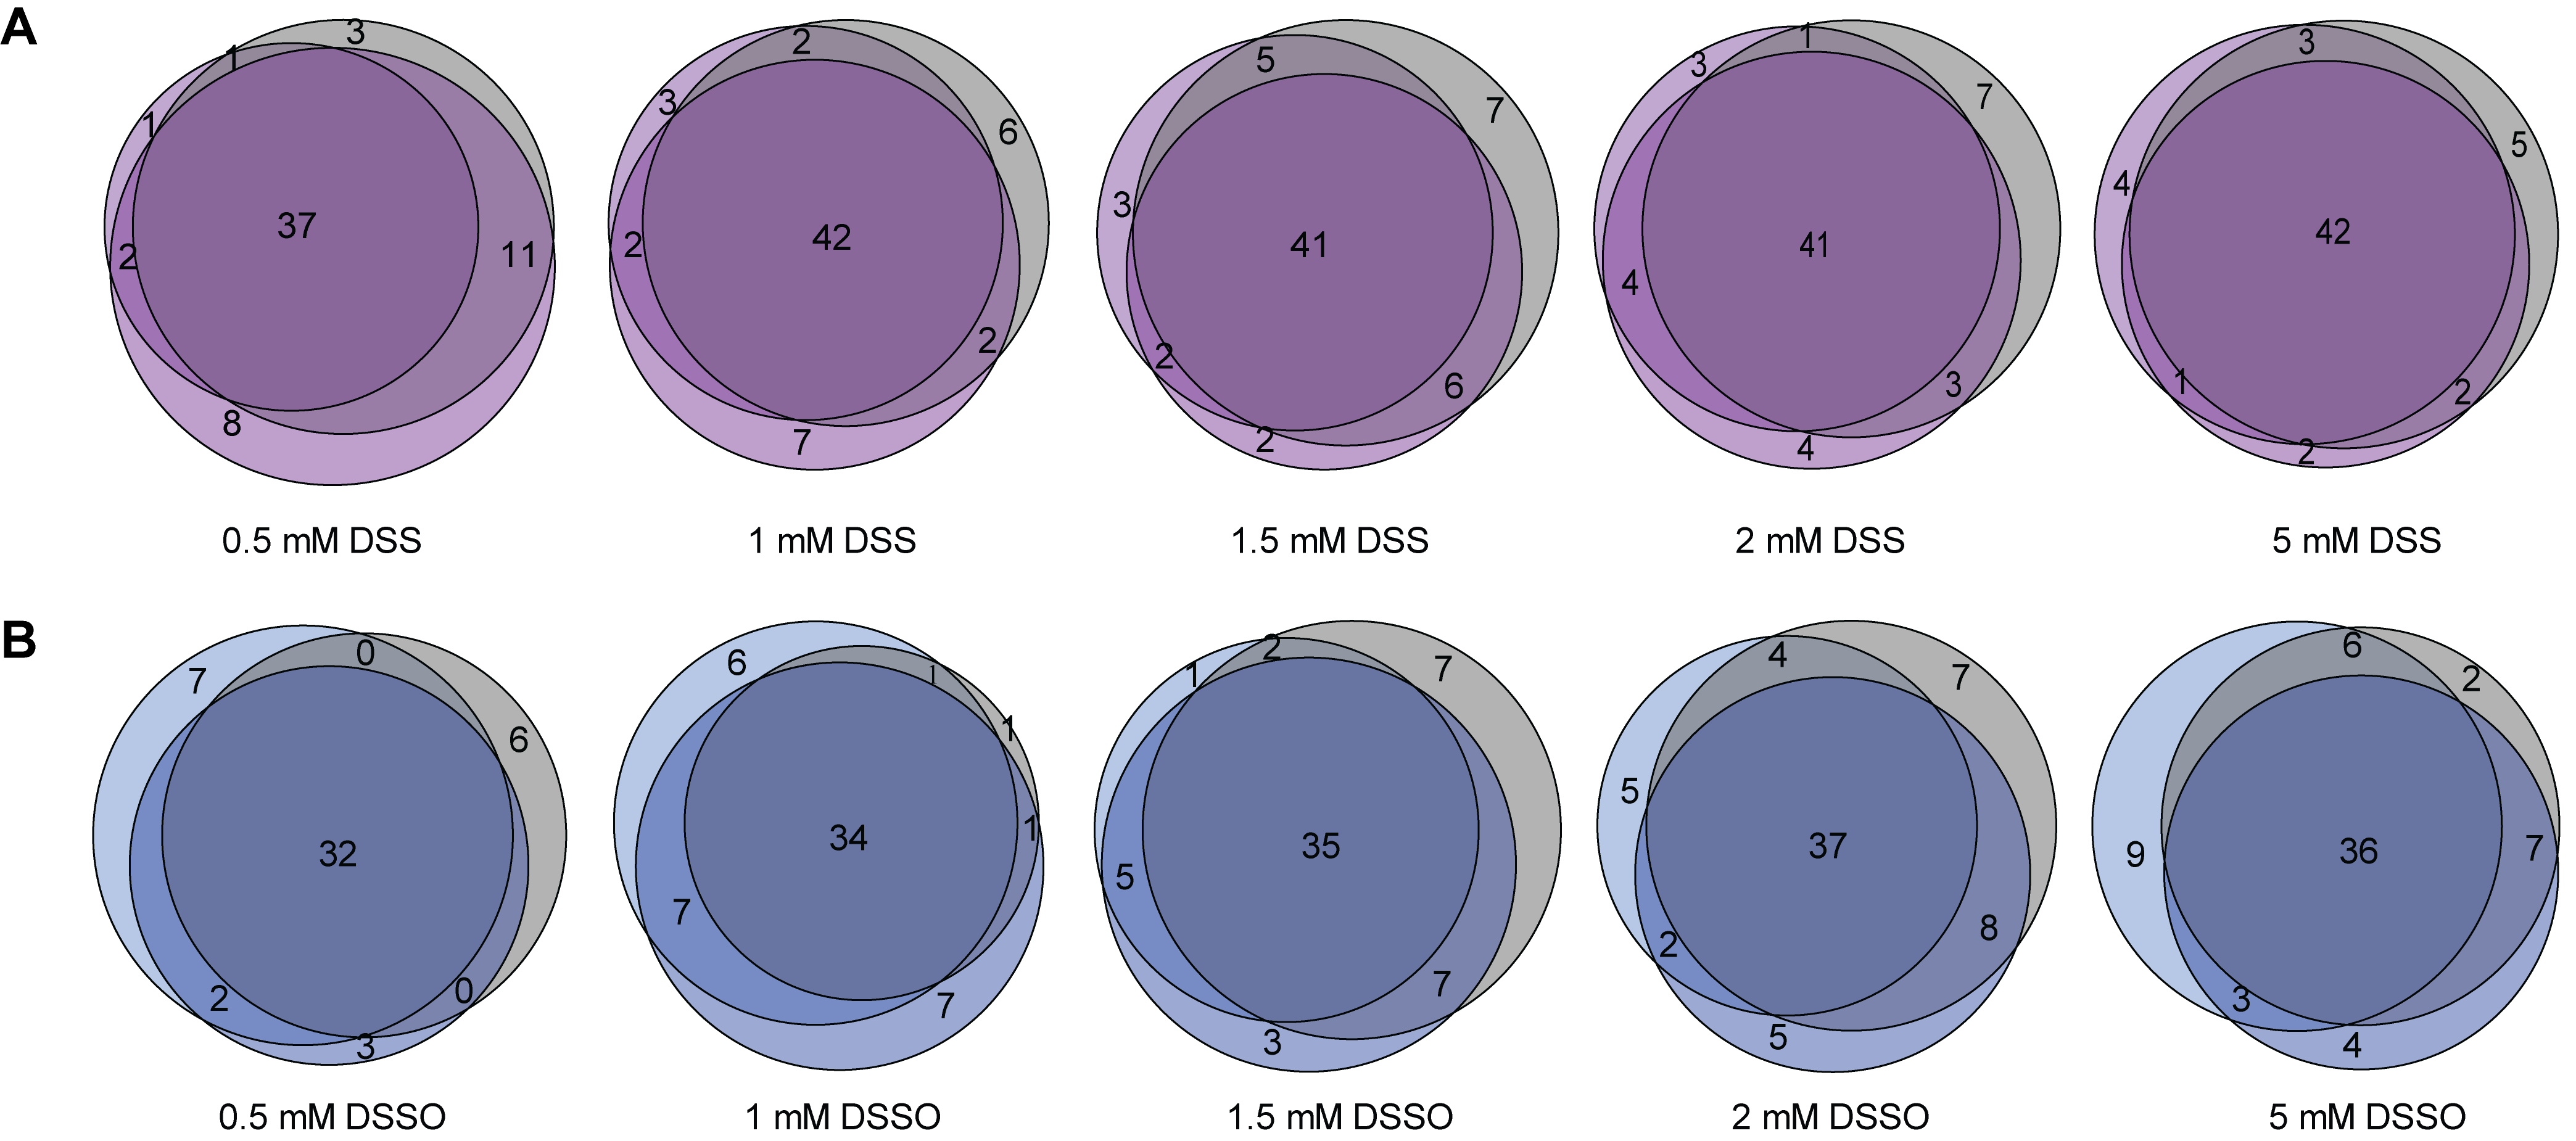
\includegraphics[width=\textwidth]{Chapter.2/Figures/SI_Fig2.png} 
        \caption{\textbf{In-gel cross-linking is highly reproducible and only marginally dependent on the concentration of the reagent.} \textbf{A.} Venn diagrams displaying the overlap of detected unique cross-links in triplicate measurements of GroEL cross-linked in gel with different DSS concentrations. \textbf{B.} Venn diagrams displaying the overlap of detected unique cross-links in triplicate measurements of GroEL cross-linked in gel with different DSSO concentrations.}
        \label{fig:ch2_app_fig2}
    \end{figure*}

    \clearpage

    \begin{figure*}[hbt!]
        \center
        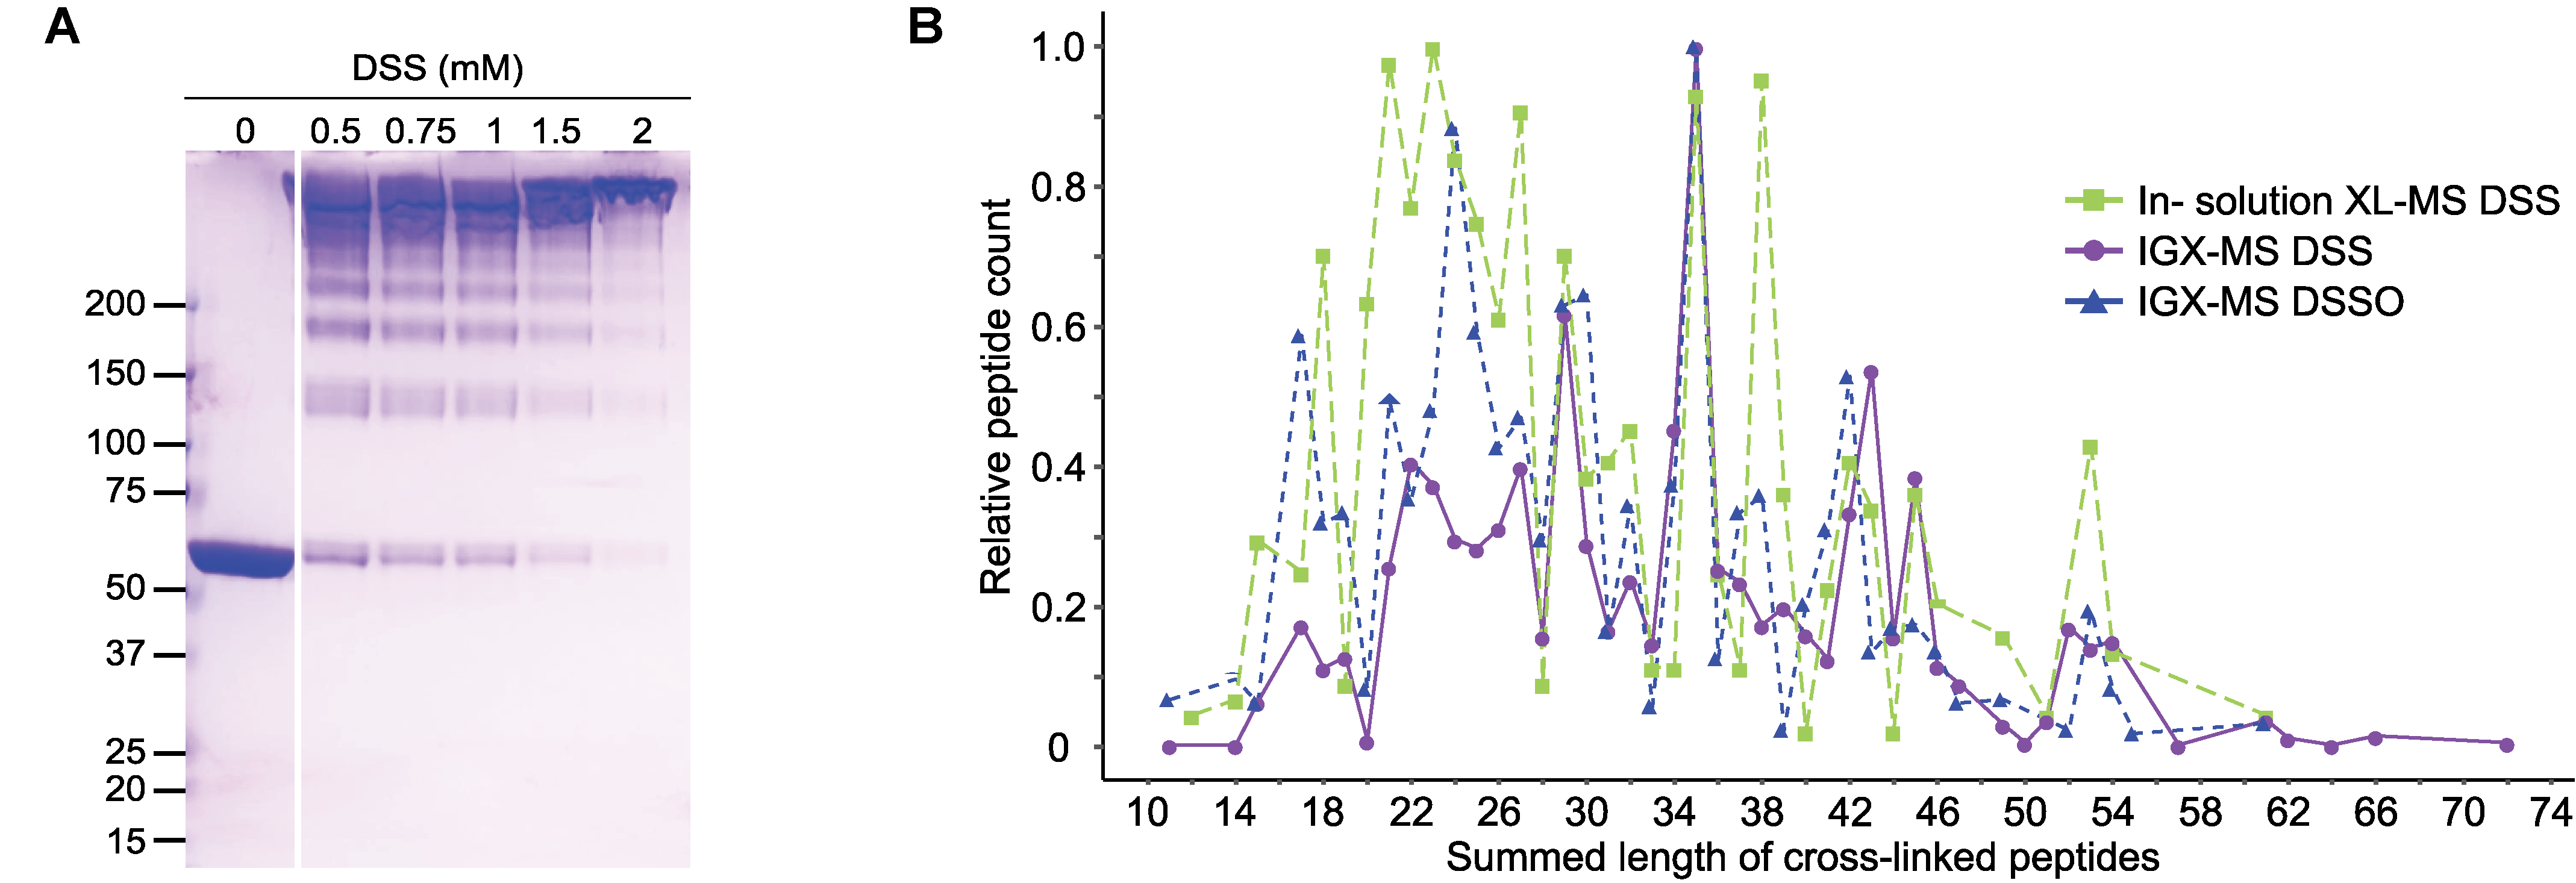
\includegraphics[width=\textwidth]{Chapter.2/Figures/SI_Fig3.png} 
        \caption{\textbf{Optimization of cross-linker concentration for in-solution XL-MS and observed cross-linked peptide length distributions for IGX-MS and in-solution XL-MS.} \textbf{A.} GroEL was cross-linked in-solution using different DSS concentrations for the optimization of the cross- linker concentration. The samples were then loaded onto a SDS-PAGE for visualization. A concentration of
        0.75 mM DSS was selected for further experiments. \textbf{B.} Comparison of summed length of cross-linked peptide-pairs from IGX-MS (1.5 mM DSS or 2 mM DSSO) or in-solution XL-MS (0.75 mM DSS) experiments.}
        \label{fig:ch2_app_fig3}
    \end{figure*}

    \begin{figure*}[hbt!]
        \center
        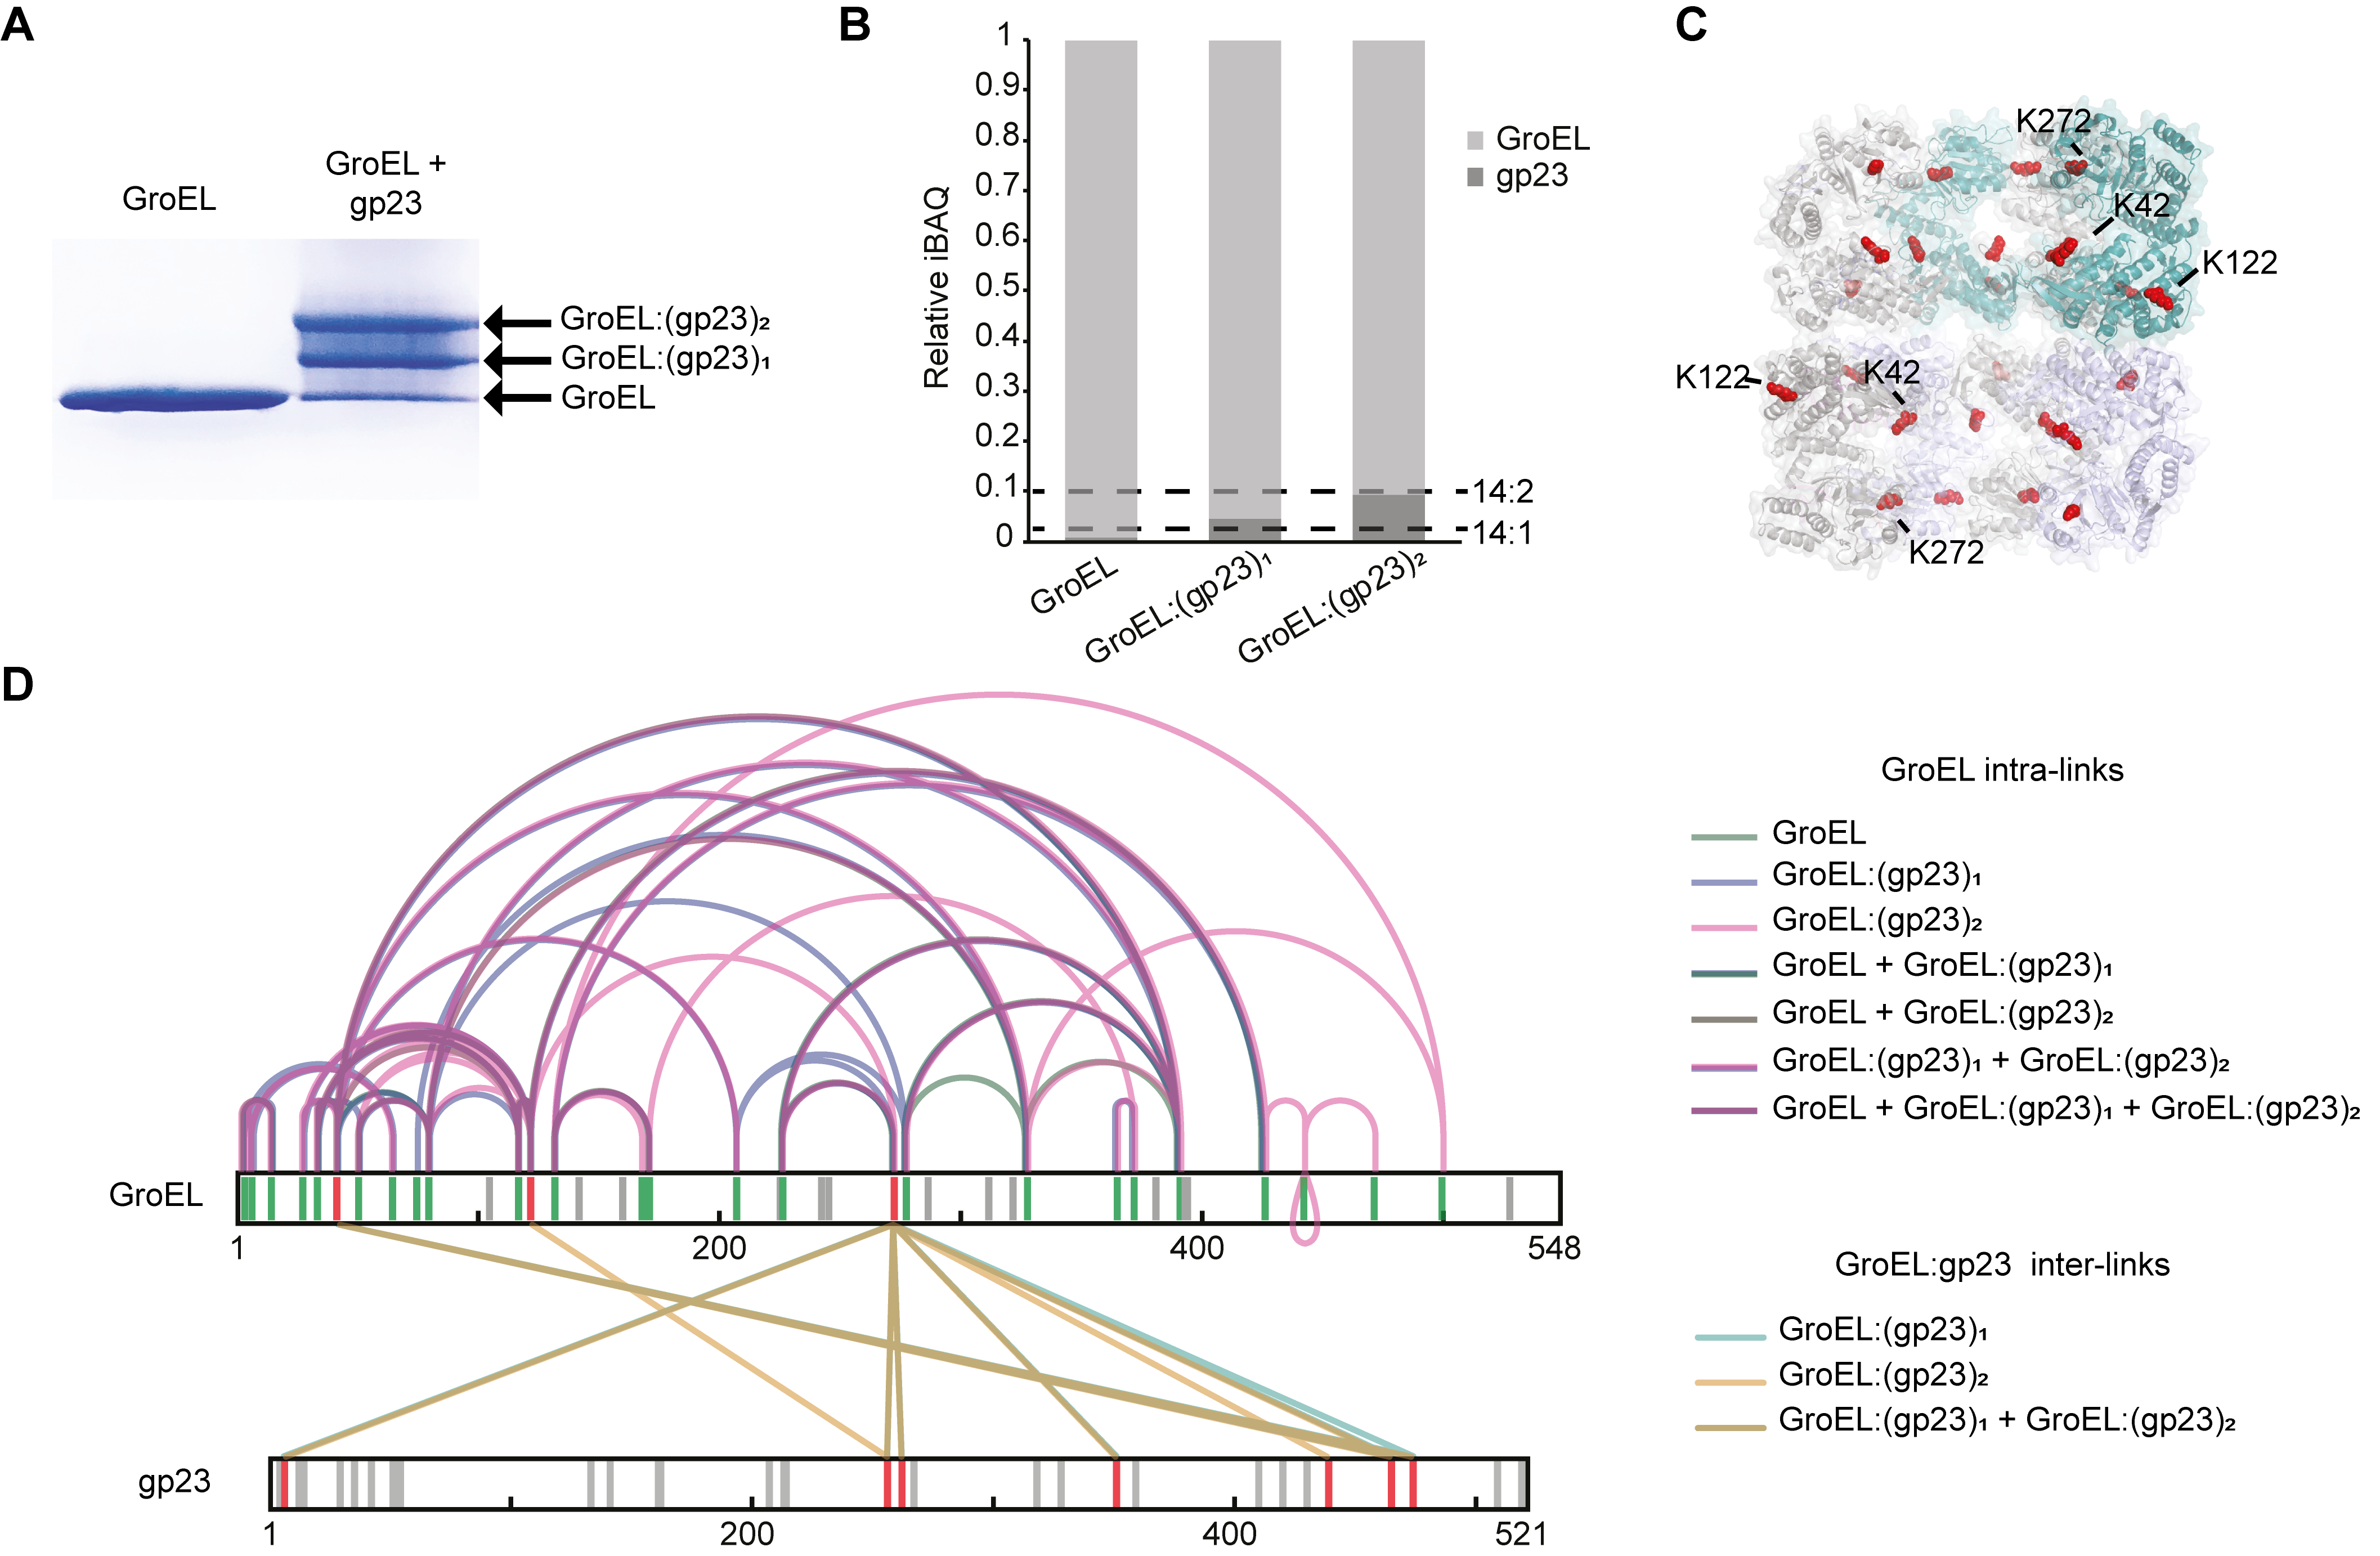
\includegraphics[width=\textwidth]{Chapter.2/Figures/SI_Fig4.png} 
        \caption{\textbf{IGX-MS of GroEL bound to the gp23 substrate.} \textbf{A.} BN-PAGE of GroEL incubated with or without unfolded gp23. The arrows indicate free GroEL or GroEL bound to one or two molecules of gp23. \textbf{B.} Label-free quantification for the estimation of the stoichiometry of the formed complexes. Relative iBAQ values of GroEL and gp23 in the three bands. Dashed lines indicate the GroEL:gp23 ratios for the theoretically expected 14:1 and 14:2 ratios. \textbf{C.} Cross-section of the structural model of GroEL (PDB ID: 1KP8) with lysine residues that were found to be cross-linked to gp23 shown in red spheres. \textbf{D.} Overlay of cross-links identified in the three bands, representing the GroEL, the GroEL:gp23, and GroEL:(gp23)2 complex. GroEL intra-links are colored green, purple, and pink. Inter-links are colored turquoise and sand. For clarity, intra-links in gp23 are not depicted. Grey lines in the sequence indicate lysine residues not cross-linked, red lines indicate inter-linked lysine residues, and green lines indicate intra-linked residues.}
        \label{fig:ch2_app_fig4}
    \end{figure*}

\end{subappendices}

\clearpage
\section*{References}
\bibliographystyle{Style_settings/bibstyle_pnas}
\bibliography{Chapter.2/chapter2_bib_form}